\documentclass[12pt]{article}
\usepackage[utf8]{inputenc}
\usepackage{amsmath, amssymb}
\usepackage{xcolor}
\usepackage{geometry}
\usepackage{hyperref}
\usepackage{fancyhdr}
\usepackage{enumitem}
\usepackage{minted} % Code highlighting
\usepackage{booktabs} % Clean tables
\usepackage{tikz} % Optional for concept maps

\geometry{margin=1in}
\hypersetup{colorlinks=true, linkcolor=blue, urlcolor=cyan}

\pagestyle{fancy}
\fancyhf{}
\fancyhead[L]{\textbf{\TOPICTITLE}}
\fancyhead[R]{\thepage}

% -------------------------------
% Topic Metadata
% -------------------------------
\newcommand{\TOPICTITLE}{Application Layer: Video Streaming and CDNs}
\title{\TOPICTITLE\\\large Study-Ready Notes}
\author{Compiled by Andrew Photinakis}
\date{\today}

\setlength{\headheight}{15pt}

\begin{document}
\maketitle
\tableofcontents
\newpage

% This LaTeX file should be saved at: computer_networks/week06/application_layer_video_streaming_cdns.tex

\textcolor{blue}{[Summary: The application layer encompasses various network services and protocols including web, email, DNS, and multimedia streaming. Video streaming and CDNs represent key modern applications addressing scalability and quality challenges.]}

\section{Video Streaming and CDNs: Context}
\begin{itemize}
    \item Stream video traffic: Major consumer of Internet bandwidth
          \begin{itemize}
              \item Netflix, YouTube, Amazon Prime: 80\% of residential ISP traffic (2020)
          \end{itemize}

    \item \textbf{Challenge: Scale} - How to reach $\sim$1 billion users?
    \item \textbf{Challenge: Heterogeneity}
          \begin{itemize}
              \item Different users have different capabilities
              \item Wired versus mobile connections
              \item Bandwidth-rich versus bandwidth-poor users
          \end{itemize}

    \item \textbf{Solution:} Distributed, application-level infrastructure
\end{itemize}

\textcolor{blue}{[Summary: Video streaming dominates Internet traffic and faces challenges of massive scale and diverse user conditions, solved through distributed infrastructure like CDNs.]}

\section{Multimedia: Video Fundamentals}

\subsection{Video Basics}
\begin{itemize}
    \item Video: Sequence of images displayed at constant rate
          \begin{itemize}
              \item Example: 24 images/second (frames per second)
          \end{itemize}

    \item Digital image: Array of pixels
          \begin{itemize}
              \item Each pixel represented by bits
          \end{itemize}

    \item Coding: Use redundancy \textit{within} and \textit{between} images to decrease bits needed
\end{itemize}

\subsection{Video Compression Techniques}
\begin{itemize}
    \item \textbf{Spatial coding} (within image):
          \begin{itemize}
              \item Instead of sending $N$ values of same color (all purple), send only two values:
              \item Color value (\textit{purple}) and number of repeated values ($N$)
          \end{itemize}

    \item \textbf{Temporal coding} (from one image to next):
          \begin{itemize}
              \item Instead of sending complete frame at $i+1$, send only differences from frame $i$
          \end{itemize}
\end{itemize}

\subsection{Video Encoding Standards}
\begin{itemize}
    \item \textbf{CBR} (Constant Bit Rate): Video encoding rate fixed
    \item \textbf{VBR} (Variable Bit Rate): Video encoding rate changes as spatial/temporal coding changes
    \item Examples:
          \begin{itemize}
              \item MPEG 1 (CD-ROM): 1.5 Mbps
              \item MPEG 2 (DVD): 3-6 Mbps
              \item MPEG 4 (Internet): 64 Kbps – 12 Mbps
          \end{itemize}
\end{itemize}

\textcolor{orange}{[Mnemonic: S-T-V - Spatial (within frame), Temporal (between frames), Variable bit rate]}
\textcolor{blue}{[Summary: Video compression uses spatial (within frame) and temporal (between frames) redundancy reduction. Encoding can be constant or variable bit rate depending on content complexity.]}

\section{Streaming Stored Video}

\subsection{Basic Scenario}
\begin{figure}[h]
    \centering
    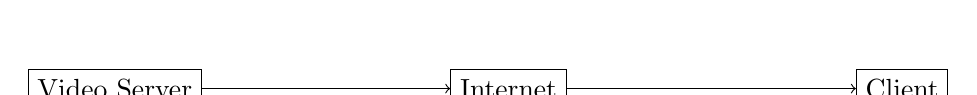
\begin{tikzpicture}[node distance=2cm]
        \node[draw, rectangle] (server) {Video Server};
        \node[draw, rectangle, right of=server, xshift=3cm] (internet) {Internet};
        \node[draw, rectangle, right of=internet, xshift=3cm] (client) {Client};
        \draw[->] (server) -- (internet);
        \draw[->] (internet) -- (client);
    \end{tikzpicture}
    \caption{Basic video streaming architecture}
\end{figure}

\subsection{Main Challenges}
\begin{itemize}
    \item Server-to-client bandwidth \textit{varies} over time due to network congestion
          \begin{itemize}
              \item Congestion can occur in home network, access network, network core, or video server
          \end{itemize}

    \item Packet loss and delay due to congestion affect:
          \begin{itemize}
              \item Playout timing (delays)
              \item Video quality
          \end{itemize}
\end{itemize}

\subsection{Streaming Process}
\begin{itemize}
    \item Video sent from server through network
    \item Network delay affects arrival timing
    \item Video received and played out at client (e.g., 30 frames/sec)
    \item \textbf{Streaming:} Client plays early part while server sends later part simultaneously
\end{itemize}

\textcolor{blue}{[Summary: Video streaming involves simultaneous transmission and playback, facing challenges of variable network conditions that affect timing and quality.]}

\section{Streaming Stored Video: Technical Challenges}

\subsection{Continuous Playout Constraint}
\begin{itemize}
    \item During client video playout, timing must match original recording timing
    \item Network delays are variable (jitter)
    \item \textbf{Solution:} Client-side buffer to compensate for jitter
\end{itemize}

\subsection{Additional Challenges}
\begin{itemize}
    \item Client interactivity:
          \begin{itemize}
              \item Pause, fast-forward, rewind, jump through video
          \end{itemize}
    \item Video packets may be lost and require retransmission
\end{itemize}

\subsection{Playout Buffering Mechanism}
\begin{figure}[h]
    \centering
    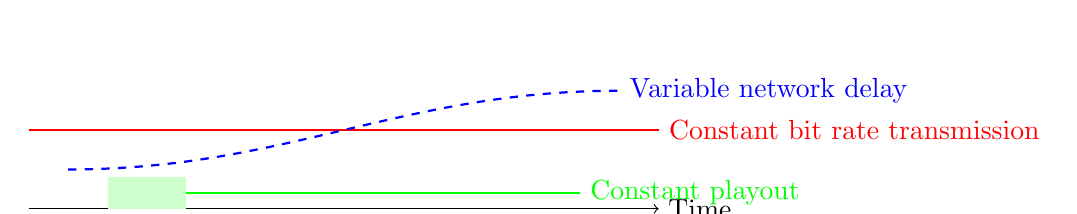
\begin{tikzpicture}
        \draw[->] (0,0) -- (8,0) node[right] {Time};
        \draw[thick, red] (0,1) -- (8,1) node[right] {Constant bit rate transmission};
        \draw[thick, blue, dashed] (0.5,0.5) to[out=0,in=180] (7.5,1.5) node[right] {Variable network delay};
        \draw[thick, green] (1,0.2) -- (7,0.2) node[right] {Constant playout};
        \fill[green!20] (1,0) rectangle (2,0.4) node[midway] {Buffer};
    \end{tikzpicture}
    \caption{Playout buffering compensates for network delay variations}
\end{figure}

\begin{itemize}
    \item Client-side buffering and playout delay compensate for:
          \begin{itemize}
              \item Network-added delay
              \item Delay jitter
          \end{itemize}
\end{itemize}

\textcolor{teal}{[Concept Map: Network variability → Jitter → Buffering need → Continuous playout]}
\textcolor{blue}{[Summary: Client buffers smooth out network jitter to maintain continuous playout, while supporting user controls and handling packet loss.]}

\section{Dynamic Adaptive Streaming over HTTP (DASH)}

\subsection{DASH Server Operations}
\begin{itemize}
    \item Divides video file into multiple chunks
    \item Each chunk encoded at multiple different rates
    \item Different rate encodings stored in different files
    \item Files replicated in various CDN nodes
    \item \textbf{Manifest file:} Provides URLs for different chunks
\end{itemize}

\subsection{DASH Client Operations}
\begin{itemize}
    \item Periodically estimates server-to-client bandwidth
    \item Consults manifest, requests one chunk at a time
    \item Chooses maximum coding rate sustainable given current bandwidth
    \item Can choose different coding rates at different times
    \item Can request from different servers
\end{itemize}

\subsection{Client Intelligence in DASH}
\begin{itemize}
    \item \textbf{When} to request chunk:
          \begin{itemize}
              \item Prevents buffer starvation or overflow
          \end{itemize}

    \item \textbf{What encoding rate} to request:
          \begin{itemize}
              \item Higher quality when more bandwidth available
          \end{itemize}

    \item \textbf{Where} to request chunk:
          \begin{itemize}
              \item From URL server "close" to client
              \item Or from server with high available bandwidth
          \end{itemize}
\end{itemize}

\textbf{Streaming video} = Encoding + DASH + Playout buffering

\textcolor{orange}{[Mnemonic: C-W-W - Chunk, When, What, Where - Client decides these three aspects]}
\textcolor{blue}{[Summary: DASH adapts video quality dynamically by breaking content into chunks encoded at multiple rates, with clients intelligently selecting optimal chunks based on current network conditions.]}

\section{Content Distribution Networks (CDNs)}

\subsection{The Scaling Challenge}
\begin{itemize}
    \item How to stream content (from millions of videos) to hundreds of thousands of \textit{simultaneous} users?
\end{itemize}

\subsection{Option 1: Single Mega-Server}
\begin{itemize}
    \item Single point of failure
    \item Point of network congestion
    \item Long (and possibly congested) paths to distant clients
    \item \textbf{Conclusion:} This solution doesn't scale
\end{itemize}

\subsection{Option 2: CDN - Distributed Approach}
\begin{itemize}
    \item Store/serve multiple copies of videos at multiple geographically distributed sites
    \item Two deployment strategies:

          \begin{itemize}
              \item \textbf{Enter Deep:} Push CDN servers deep into many access networks
                    \begin{itemize}
                        \item Close to users
                        \item Example: Akamai - 240,000 servers in >120 countries (2015)
                    \end{itemize}

              \item \textbf{Bring Home:} Smaller number (10's) of larger clusters in POPs near access networks
                    \begin{itemize}
                        \item Example: Limelight
                    \end{itemize}
          \end{itemize}
\end{itemize}

\subsection{CDN Operation Process}
\begin{enumerate}
    \item CDN stores copies of content at CDN nodes
    \item Subscriber requests content, service provider returns manifest
    \item Using manifest, client retrieves content at highest supportable rate
    \item May choose different rate or copy if network path congested
\end{enumerate}

\subsection{Over-the-Top (OTT) Challenges}
\begin{itemize}
    \item OTT: "Over the Top" - Internet host-host communication as service
    \item Key challenges coping with congested Internet from the "edge":
          \begin{itemize}
              \item What content to place in which CDN node?
              \item From which CDN node to retrieve content?
              \item At which rate to retrieve content?
          \end{itemize}
\end{itemize}

\textcolor{teal}{[Concept Map: Scaling problem → Single server fails → Distributed CDN solution → Enter deep/Bring home strategies → Manifest-based adaptive delivery]}
\textcolor{blue}{[Summary: CDNs solve scaling challenges through geographically distributed content replication, with strategies focusing on proximity to users and intelligent content delivery decisions.]}

\section*{Exam Questions}

\subsection*{Video Fundamentals}
\begin{enumerate}
    \item Compare and contrast spatial versus temporal video coding, providing examples of each.
    \item What are the advantages of VBR over CBR for video encoding? When might CBR be preferred?
    \item Explain how both spatial and temporal coding reduce the bitrate required for video transmission.
\end{enumerate}

\subsection*{Streaming Challenges}
\begin{enumerate}
    \item Describe the "continuous playout constraint" and explain how client-side buffering addresses it.
    \item What network factors can cause variations in video streaming quality, and how do they manifest to the end user?
    \item Why is simple retransmission of lost packets problematic for real-time video streaming?
\end{enumerate}

\subsection*{DASH and Adaptive Streaming}
\begin{enumerate}
    \item Explain the three key decisions a DASH client must make for each video chunk request.
    \item How does the manifest file enable adaptive bitrate streaming in DASH?
    \item What metrics might a DASH client use to determine the appropriate encoding rate to request?
\end{enumerate}

\subsection*{CDNs and Distribution}
\begin{enumerate}
    \item Compare the "enter deep" and "bring home" CDN deployment strategies, including advantages of each.
    \item Explain how a CDN helps overcome the scaling limitations of a single mega-server approach.
    \item What are the main OTT challenges in content distribution, and how do CDNs address them?
\end{enumerate}

\textcolor{red}{[Exam Questions: Comprehensive coverage of video encoding, streaming challenges, adaptive streaming, and CDN architectures with practical application scenarios.]}


\end{document}